\chapter{O que foi apagado}\label{cap:apagado}

O capítulo anterior mediu o mundo que não foi observado. Este mede o espelho dele: o que o registro
teve e já não tem, porque a memória do sistema foi jogada fora. A pergunta é se há preço que traga o
passado de volta.

\section{A tentativa que explode}

O sistema mais simples que esquece é $x(t) = a\,x(t-1) + \eta(t)$, com \emph{a} entre zero e um.
Com \emph{a} perto de um a memória é longa; com \emph{a} perto de zero o processo esquece tudo num
passo. A escala do processo é $\sigma_x = \sigma/\sqrt{1-a^2}$, e a memória dele é $1/(1-a)$ dias, com a
escala do ruído em \numApagadoSigma{}.

A tentativa que vem à cabeça é desfazer o decaimento: dividir o estado de hoje por \emph{a}, uma vez
para cada dia que se quer andar para trás. Medida em \numApagadoDias{} dias por mundo, em
\numApagadoSementes{} mundos, ela já erra no primeiro passo --- \numApagadoInversoNoventaCentesimos{}
com \emph{a} em \numApagadoADoTeste{} ---, e daí em diante cresce sem teto: a
\numApagadoDiasMaior{} dias para trás o número que sai não é um erro, é lixo aritmético.

O motivo é simples e vale a pena ser dito: cada passo para trás divide por \emph{a} o erro
acumulado **e** o ruído desconhecido que entrou naquele passo. O ruído entra com o sinal do sinal e
sai multiplicado.

\section{As duas reconstruções}

\begin{proposicao}[o erro de cada reconstrução]\label{prop:reconstrucao}
Para o processo $x(t) = a\,x(t-1) + \eta(t)$, com $\eta$ de variância $\sigma^2$ e $0<a<1$:
a reconstrução pelo mapa inverso, feita \emph{k} dias para trás a partir do estado de hoje, tem erro
\quad $\sigma\sqrt{(1-a^{2k})/(1-a^2)}\big/a^{k}$; \quad e a reconstrução ótima --- a esperança
condicional, que encolhe o estado de hoje por $a^{k}$ --- tem erro $\sigma_x\sqrt{1-a^{2k}}$.
\end{proposicao}

\begin{proof}
O erro da reconstrução inversa obedece $e_{j+1} = e_j/a + \eta/a$, com $e_0 = 0$: dividir por $a$
amplifica o erro acumulado e soma o ruído do passo, também dividido por $a$. Iterando, o erro é
$\sum_{j<k} a^{j}\eta_{t-j}/a^{k}$, cuja variância é a soma geométrica da primeira forma. Para a
reconstrução ótima, a esperança de $x(t-k)$ dado $x(t)$ é $a^{k}x(t)$ num processo gaussiano
estacionário, e a variância condicional que sobra é $\sigma_x^{2}(1-a^{2k})$.
\end{proof}

As duas formas dizem coisas opostas, e é isso que decide o capítulo. A primeira cresce sem teto: a
reconstrução inversa fica cada vez pior e nunca se conserta. A segunda converge para a escala do
próprio processo --- que é o erro de quem não olha para nada. O passado **desbota** em vez de se perder num ponto, e desbota até virar palpite puro.

\begin{table}[htbp]
  \centering
  \small
  \begin{tabular}{rrrr}
    \hline
    a do & escala & erro do inverso & erro do ótimo \\
    processo & do processo & em um dia & em \numApagadoDiasMaior{} dias \\
    \hline
    \numApagadoADoTeste{} (metade) & \numApagadoEscalaMeio & \numApagadoInversoMeio & \numApagadoOtimoMeio \\
    oitenta centésimos & \numApagadoEscalaOitentaCentesimos & \numApagadoInversoOitentaCentesimos & \numApagadoOtimoOitentaCentesimos \\
    noventa centésimos & \numApagadoEscalaNoventaCentesimos & \numApagadoInversoNoventaCentesimos & \numApagadoOtimoNoventaCentesimos \\
    noventa e cinco & \numApagadoEscalaNoventaECincoCentesimos & \numApagadoInversoNoventaECincoCentesimos & \numApagadoOtimoNoventaECincoCentesimos \\
    noventa e nove & \numApagadoEscalaNoventaENoveCentesimos & \numApagadoInversoNoventaENoveCentesimos & \numApagadoOtimoNoventaENoveCentesimos \\
    \hline
  \end{tabular}
  \caption{As duas reconstruções medidas, e a escala do processo que serve de referência. Um erro
    igual à escala quer dizer que a reconstrução não sabe mais do que um palpite sorteado da
    distribuição.}
  \label{tab:reconstrucoes}
\end{table}

A primeira linha da tabela já mostra o caso extremo: com \emph{a} na metade, o mapa inverso erra
\numApagadoInversoMeio{} no primeiro passo, contra uma escala de \numApagadoEscalaMeio{}. Ele é pior
do que não fazer nada desde o primeiro dia. A reconstrução ótima, na mesma linha, termina em
\numApagadoOtimoMeio{}, que é exatamente a escala: o passado dela desbotou por completo.

\begin{figure}[htbp]
  \centering
  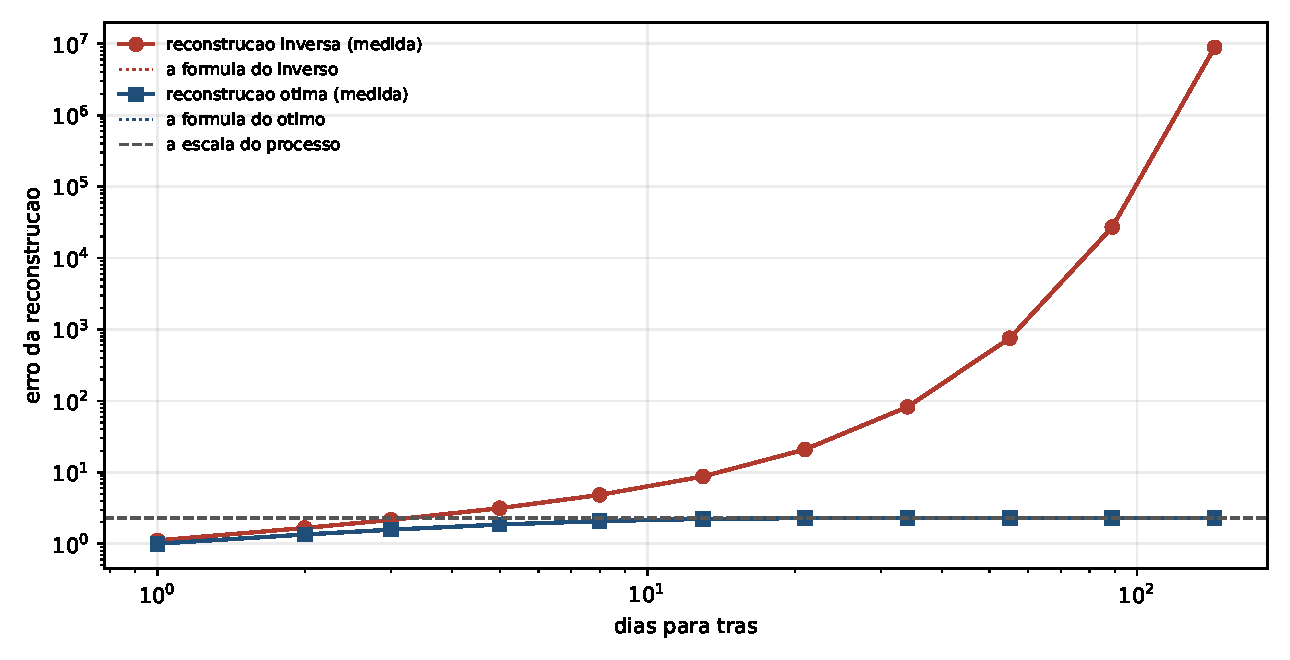
\includegraphics[width=\linewidth]{figuras/E16_o_que_foi_apagado_1.pdf}
  \caption{O erro das duas reconstruções contra os dias para trás, com a escala do processo como
    linha de referência. Os pontos são medidos e as linhas pontilhadas são as formas fechadas da
    \cref{prop:reconstrucao}.}
  \label{fig:reconstrucoes}
\end{figure}

\section{O horizonte, e o que ele não é}

Se o passado desbota em vez de sumir, então "até onde ele volta" é uma escolha declarada, e a
escolha é a tolerância: quanto de erro se aceita, em fração da escala do processo. Com ela, o
horizonte sai da conta: $\log(1-\theta^{2})$ dividido por $2\log a$ dias.

\begin{table}[htbp]
  \centering
  \small
  \begin{tabular}{rrrr}
    \hline
    a do & memória do & horizonte de & horizonte de \\
    processo & processo & tolerância estreita & tolerância larga \\
    \hline
    metade & \numApagadoMemoriaMeio & \numApagadoHorizonteMeio & \numApagadoHorizonteLargoMeio \\
    oitenta centésimos & \numApagadoMemoriaOitentaCentesimos & \numApagadoHorizonteOitentaCentesimos & \numApagadoHorizonteLargoOitentaCentesimos \\
    noventa centésimos & \numApagadoMemoriaNoventaCentesimos & \numApagadoHorizonteNoventaCentesimos & \numApagadoHorizonteLargoNoventaCentesimos \\
    noventa e cinco & \numApagadoMemoriaNoventaECincoCentesimos & \numApagadoHorizonteNoventaECincoCentesimos & \numApagadoHorizonteLargoNoventaECincoCentesimos \\
    noventa e nove & \numApagadoMemoriaNoventaENoveCentesimos & \numApagadoHorizonteNoventaENoveCentesimos & \numApagadoHorizonteLargoNoventaENoveCentesimos \\
    \hline
  \end{tabular}
  \caption{O horizonte de recuperação medido, em dias, para duas tolerâncias, ao lado da memória do
    processo. As duas medidas descrevem o mesmo sistema e não são a mesma coisa.}
  \label{tab:horizontes-do-apagado}
\end{table}

A tolerância estreita é a metade da escala do processo e a larga são noventa por cento dela. As
duas colunas do meio e a primeira não coincidem, e a diferença não é detalhe. A memória do
processo diz quanto tempo a influência de um dia dura; o horizonte diz até onde o valor daquele dia
pode ser reconstruído com um erro aceitável. Com \emph{a} em noventa e nove centésimos a memória é de
\numApagadoMemoriaNoventaENoveCentesimos{} dias e o horizonte tolerante é de
\numApagadoHorizonteLargoNoventaENoveCentesimos{}: o passado ainda volta de mais longe do que a
memória sugere, e volta pior.

\begin{figure}[htbp]
  \centering
  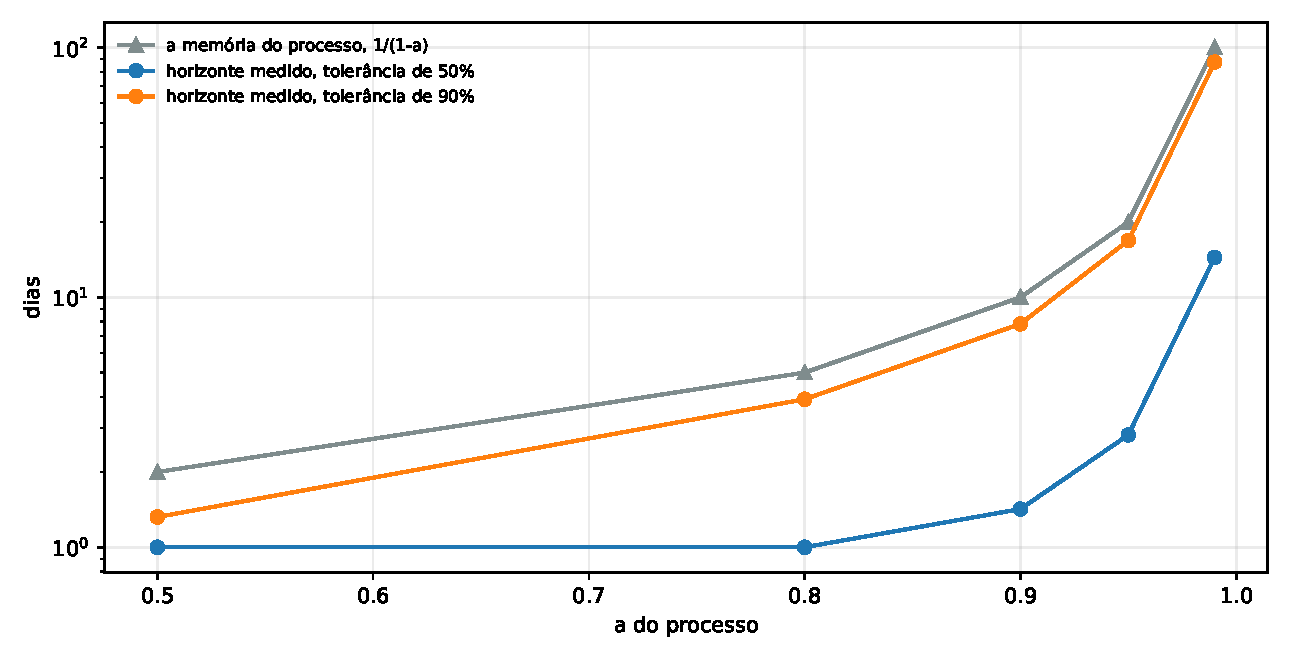
\includegraphics[width=\linewidth]{figuras/E16_o_que_foi_apagado_2.pdf}
  \caption{A memória do processo e os dois horizontes de recuperação, contra \emph{a}. São três medidas do mesmo sistema, e cada uma
    responde a uma pergunta diferente --- a curva mais alta é a da memória, e as outras duas são
    horizontes de recuperação.}
  \label{fig:horizontes}
\end{figure}

\section{Bits não compram o passado}

Falta o controle que separa o que apaga o passado do que só o embaralha. Se o que apaga fosse a
aritmética, guardar o estado com mais precisão esticaria o horizonte. O horizonte fica onde estava: guardando o estado
com \numApagadoBitsMenor{} bits, o horizonte é de \numApagadoHorizonteDeBits{} dias, e guardando com
precisão inteira ele é de \numApagadoHorizonteSemBits{} --- praticamente o mesmo número, e o mesmo
que a \cref{prop:reconstrucao} prevê, \numApagadoHorizonteDaFormula{}.

A leitura é direta: o que apaga o passado é o **ruído que entrou nele**, e não a precisão com que
ele foi guardado. Um sistema que guarda o estado em quatro bits e outro que o guarda em cinquenta e
três perdem o passado no mesmo lugar.

\section{O que fica}

Fica a resposta do segundo pedaço do andar, e ela tem uma parte que se compra e uma que fica fora do
mercado. A que fica fora é o dia que passou para trás do horizonte: ali nenhum método, nenhum bit e
nenhuma paciência trazem o valor de volta, porque a informação já saiu do estado. A parte que se compra é
o horizonte maior --- e ele se compra de duas maneiras, ambas declaradas: com um processo de memória
mais longa, e com uma tolerância mais frouxa. Não há terceira.

Fica também a correção que este capítulo faz na intuição do anterior. Lá, o esquecimento era uma
taxa escolhida para acompanhar o mundo; aqui, ele aparece como o que de fato é: uma perda com
endereço. A memória que o capítulo da memória recomendou, de vinte e um dias, tem o seu horizonte de
recuperação medido, e o que ficou para trás dele não está guardado em lugar nenhum.

O terceiro pedaço do andar é o que a margem não conta. Duas medições desta espiral mostraram que proteger
cada perna no seu próprio corte não vê o que acontece entre elas; e que ler uma série só pelo
segundo momento é ler metade dela. Falta juntar as duas coisas numa conta só.
